\chapter{Further Work}
\label{chap:further-work}

Our interactions with the Synote code base have given us the opportunity to discover its existing strengths and weaknesses, as well as those introduced through our development. Existing weaknesses mostly correspond to the methodology for server side testing whereas the weaknesses we have introduced stem from learning technologies on the fly. With the knowledge we have ascertained at this point, we would propose several enhancements to Synote's design which we shall discuss as future work.

\section{Server Side Testing}
\label{subsec:server-side-testing}

Firstly, we believe that performing integration tests on \texttt{controllers} to test for situations that should be handled by \texttt{policies} is not desirable. The test shown in \textbf{Listing \ref{lst:creditcontroller-test-file}} intends to check that the user requesting to view credits is himself the credit owner; an action that is performed in a \texttt{policy} named \texttt{canListCreditHistory.js}, not the \texttt{controller}.\\

Our solution is two fold. Firstly, the \texttt{policy} file should be unit tested using mocking and spying techniques. Secondly, the controller actions should be integration tested using dependency injection with a fake database. An example of our suggested \texttt{policy} testing convention is shown in \textbf{Listing \ref{lst:can-list-credit-test}} and demonstrates how the same test (with \texttt{admin} rule extension) can be written using a mocked request stub and a \textit{Sinon} spy. This approach has the added benefit of running much faster than an HTTP request.\\

\begin{listing}[H]
\begin{minted}[xleftmargin=\parindent, linenos, breaklines, breakanywhere, bgcolor=lightgray, fontsize=\small]{js}
it('should not view credit if not credit owner himself',
  function (done) {
    var user = testdata.getUserByEmail('yl2@ecs.soton.ac.uk');
    var anotheruser = testdata.getUserByEmail('mw@ecs.soton.ac.uk');
    var access_token = testdata.getUserTokenById(anotheruser.id);
    var c;
    Credit.findOne({owner: user.id}).then(function (credit) {
      c = credit;
      return request(sails.hooks.http.app)
        .get('/credit/' + credit.id)
        .set('Authorization', "Bearer " + access_token)
        .expect(403);
    }).then(function (res) {
      done();
    }).catch(done);
});
\end{minted}
\captionof{listing}{\texttt{CreditController.test.js} Snippet}
\label{lst:creditcontroller-test-file}
\end{listing}

\begin{listing}[H]
\begin{minted}[xleftmargin=\parindent, linenos, breaklines, breakanywhere, bgcolor=lightgray, fontsize=\small]{js}
var req, res, cb;

beforeEach(function (done) {
  req = {
    user_profile: {
      id: '',
      role: ''
    },
    user: {sub: ''}
  };
  res = {};
  cb = sinon.spy();
  done();
});

it('If bearer does not match user and not admin, it is forbidden',
  function (done) {
    req.method = 'GET';
    req.user_profile.id = 'fakeid';
    req.user.sub = 'not matching fakeid';
    req.user.admin = 'not admin';
    res.forbidden = sinon.spy();
    canListCreditHitory(req, res, cb);

    expect(res.forbidden).called;
    expect(cb).not.called;
    done();
});
\end{minted}
\captionof{listing}{\texttt{canListCreditHistory.test.js} Snippet}
\label{lst:can-list-credit-test}
\end{listing}

\section{Auto Generated Page Objects}
\label{subsec:auto-generated-page-objects}

We envisioned an extension of our E2E testing framework to auto-generate page object files, but sadly it did not fall into the required feature set. The foundations for this enhancement exist in the form of our HTML ID convention such that a script could be produced to parse an HTML file and generate a page object skeleton based on element IDs. Automatic generation of required test framework skeleton files is also not limited to page objects. Partial templates for \texttt{feature} files and \texttt{step} files could also be generated as part of the envisioned script.

\section{E2E Test Reporting}
\label{subsec:e2e-test-reporting}

At present, the E2E testing framework is responsible for generating a folder hierarchy  in which to save a test report based on: the latest Synote commit hash, current deployment and the date-time at which the test suite ran. At an earlier stage the framework was also responsible for posting a link to the generated report on \textit{Slack}, but we believe the framework should not be responsible for either of these actions and consequently we have moved \textit{Slack} posting tasks to the \textit{Jenkins} CI script. The task of separating out the folder hierarchy generation still exists and is recommended as a future task.

\section{Ghost Inspector}
\label{subsec:ghost-inspector}

Our testing methodology contains a statement: \textit{If a component cannot be tested using our framework, it is considered a bug and should be changed}. In the case of \texttt{Toastr} alerts we adhered to this statement and developed an alternative alerts system. However another component, \texttt{cg-busy}, could also not be tested reliably. This component's use in Synote is desirable and consequently we implemented a test using Ghost Inspector to resolve the testing issue. Including Ghost Inspector in our E2E testing framework would be a fruitful future task resolving the need to compromise on component use.

\section{Testing Database}
\label{subsec:testing-database}

An ongoing point of concern with our E2E testing framework is how the deployment database is affected by E2E tests. Our current approach is to use hooks to prepare and restore database records for each test case, which is necessary for SILO tests. We achieved this by implementing and making calls to a \texttt{controller} on Synote's server. We are uncomfortable with this solution because it tightly couples the testing framework to the system under test, but had to proceed with this method in order to progress.\\

A proposal for future enhancement could be to make temporary deployments on which to run the E2E tests, thus not affecting the real deployment database. Then, if all tests pass, the deployment can be performed as a permanent deployment over the existing real version. In this circumstance, the current method of migrating the database could also be used to seed data used in tests removing the need to use a server side \texttt{controller}.

\section{Server Side Design}
\label{subsec:server-side-design}

Given what we have learned of \textit{Sails} and \textit{Stripe}, we also have some thoughts on how to improve our implementation of the payment system. One suggestion is to improve the DB design by not storing \textit{stringified} JSONs, but instead creating tables similar to those shown in \textbf{Figure \ref{fig:proposed-schema}}. The \texttt{source} table has the additional benefit of decoupling customer objects from the \texttt{User} table and the \texttt{Transaction} table replaces \texttt{CreditHistory} table, which facilitates providing more detailed transaction information to the \textit{Credits History} view.\\

\begin{figure}[!hbt]
  \centering
 	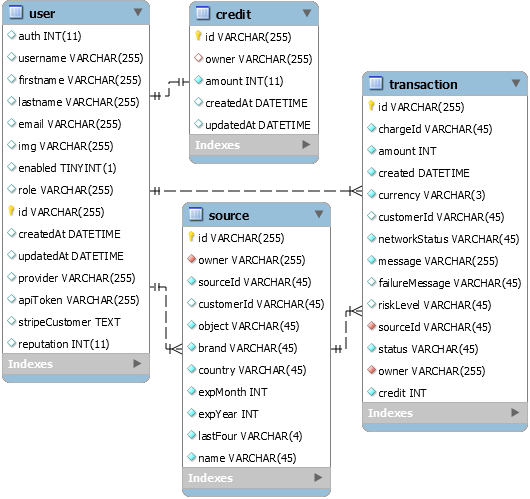
\includegraphics[width=\textwidth]{proposed-schema.png}
  \caption{Proposed Design}
 	\label{fig:proposed-schema}
\end{figure}

Additionally, our implementation has not included a function to perform refunds which this DB design would be able to record in the \texttt{transaction} table. Lastly, our payment system could also be improved to handle error cases involving declined cards and fraud, which again have been catered for with respect to logging through the \texttt{transaction} table design.
